% XCircuit output "cmos_inverter.tex" for LaTeX input from cmos_inverter.eps
\def\putbox#1#2#3#4{\makebox[0in][l]{\makebox[#1][l]{}\raisebox{\baselineskip}[0in][0in]{\raisebox{#2}[0in][0in]{\scalebox{#3}{#4}}}}}
\def\rightbox#1{\makebox[0in][r]{#1}}
\def\centbox#1{\makebox[0in]{#1}}
\def\topbox#1{\raisebox{-0.60\baselineskip}[0in][0in]{#1}}
\def\midbox#1{\raisebox{-0.20\baselineskip}[0in][0in]{#1}}
   \scalebox{1}{
   \normalsize
   \parbox{1.64583in}{
   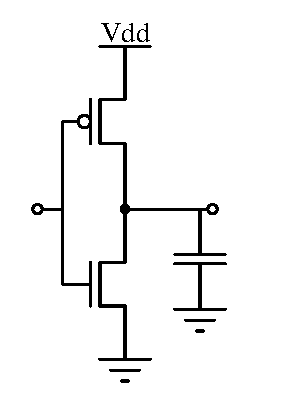
\includegraphics[scale=1]{cmos_inverter}\\
   % translate x=416 y=316 scale 0.38
   \putbox{1.39in}{1.20in}{1.20}{out}%
   \putbox{0.06in}{1.29in}{1.20}{in}%
   \putbox{1.47in}{0.79in}{1.20}{$\text{C}_\text{L}$}%
   } % close 'parbox'
   } % close 'scalebox'
   \vspace{-\baselineskip} % this is not necessary, but looks better
